\documentclass[letterpaper,10pt]{article}

\usepackage{listings}
\usepackage{color}
\usepackage{tikz}
\usepackage{caption}

\setlength{\headheight}{0in}
\setlength{\marginparsep}{0in}
\setlength{\footskip}{0in}
\setlength{\headsep}{0in}
\setlength{\marginparwidth}{0in}
\setlength{\marginparpush}{0in}
\setlength{\voffset}{0in}
\setlength{\hoffset}{-1in}
\setlength{\voffset}{-1in}
\setlength{\oddsidemargin}{0.75in}
\setlength{\evensidemargin}{0.75in}
\setlength{\topmargin}{0.75in}
\setlength{\textheight}{9.5in}
\setlength{\textwidth}{7in}
\setlength{\parindent}{0in}
\setlength{\parskip}{10pt} %change this to match font size

\pagestyle{empty}
\definecolor{gray}{gray}{0.75}
\usetikzlibrary{shapes,arrows,calc}
\lstset{backgroundcolor=\color{gray},frame=single}

% define block styles
\tikzstyle{line} = [draw, -latex']
\tikzstyle{block} = [draw, rectangle, text centered, minimum height=2em]
\tikzstyle{mlblock} = [draw, rectangle, text width=10em, text centered, minimum height=2em]
\tikzstyle{decision} = [draw, diamond, text width=4.5em, text centered, node distance=3cm, inner sep=0pt]
\tikzstyle{cloud} = [draw, rectangle, text centered, rounded corners, minimum height=2em]

\begin{document}
    Albert Chang and Nipun Chopra\\
    CSE-380 A6\\
    University at Buffalo\\
    Dr. Kris Schindler\\
    March 1, 2011\\
    \textit{Lab 4 Documentation}

    The objective of Lab 4 was to learn about using the general purpose
    input/output, GPIO, and how to factor code using \textbf{export} and
    \textbf{extern}. There are two parts to the program.

    First the user pushes each of the four push buttons. As the buttons are
    pushed, the corresponding LEDs light up. After each individual button has
    been pushed once, the program moves onto the second part of the program.

    The second part makes use of the UART. The user enters in a hexadecimal,
    0-9, a-f, and A-F, and it is printed on the seven-segment display. Upon
    writing either Q or q, the program quits.

    The user is given feedback by the RGB LED. When the program is waiting for
    push button input, it lights green. When the user pushes a button, it
    lights blue. When it is waiting for UART input, it lights white. Finally,
    when it exits, it lights red.

    Half of the routines were written in the previous labs. Their respective
    flowcharts are shown in Figs. \ref{flo:uart_init}, \ref{flo:chars},
    \ref{flo:output_string}, and \ref{flo:read_string}.

    \begin{figure}[p]
        \begin{center}
    \begin{tikzpicture}[node distance = 3cm, auto]
        \node[cloud] (origin) {Start};
        \node[block, below of=origin, node distance=1.5cm] (enable) {Write 0x5 to PINSEL0 to enable UART0};
        \node[mlblock, below of=enable] (init) {Configure U0LCR:\\%
                                                8-bit word length\\%
                                                1 stop bit\\%
                                                no parity\\%
                                                disable break control\\%
                                                enable access latch};
        \node[block, below of=init] (baud) {Set baud rate to 9600};
        \node[mlblock, below of=baud] (conf) {Configure U0LCR:\\%
                                                8-bit word length\\%
                                                1 stop bit\\%
                                                no parity\\%
                                                disable break control\\%
                                                disable latch access};
        \node[cloud, below of=conf] (stop) {Stop};
        \path[line] (origin) -- (enable);
        \path[line] (enable) -- (init);
        \path[line] (init) -- (baud);
        \path[line] (baud) -- (conf);
        \path[line] (conf) -- (stop);
    \end{tikzpicture}
\end{center}

        \caption{Flowchart of \textit{uart\_init} routine.}
        \label{flo:uart_init}
    \end{figure}

    \begin{figure}[p]
        \begin{minipage}{0.5\linewidth}
            \begin{center}
    \begin{tikzpicture}[node distance = 1.5cm, auto]
        \node[cloud] (origin) {Start};
        \node[decision, below of=origin] (test) {Test THRE in status register};
        \node[block, below of=test, node distance = 3.5cm] (store) {Store byte in transmit register};
        \node[cloud, below of=store] (stop) {Stop};
        \path[line] (origin) -- (test);
        \path[line] (test) -- node [near start] {1} (store);
        \path[line] (test) -| node [near start] {0} +(3,2.25) -- +(0,2.25);
        \path[line] (store) -- (stop);
    \end{tikzpicture}
\end{center}

        \end{minipage}%
        \begin{minipage}{0.5\linewidth}
            \begin{center}
    \begin{tikzpicture}[node distance = 1.5cm, auto]
        \node[cloud] (origin) {Start};
        \node[decision, below of=origin] (test) {Test RDR in status register};
        \node[block, below of=test, node distance = 3.5cm] (read) {Read byte from receive register};
        \node[cloud, below of=read] (stop) {Stop};
        \path[line] (origin) -- (test);
        \path[line] (test) -- node [near start] {1} (read);
        \path[line] (test) -| node [near start] {0} +(3,2) -- +(0,2);
        \path[line] (read) -- (stop);
    \end{tikzpicture}
\end{center}

        \end{minipage}
        \caption{Flowcharts of \textit{output\_char} (left) and \textit{read\_char} (right) routines.}
        \label{flo:chars}
    \end{figure}

    \begin{figure}[p]
        \begin{center}
    \begin{tikzpicture}[node distance = 1.5cm, auto]
        \node[cloud] (origin) {Start};
        \node[block, below of=origin] (read) {Load byte from memory};
        \node[decision, below of=read] (null) {Is it the null character?};
        \node[block, right of=null, node distance=5cm] (output) {Output character};
        \node[cloud, below of=null, node distance=3cm] (stop) {Stop};
        \path[line] (origin) -- (read);
        \path[line] (read) -- (null);
        \path[line] (null) -- node [near start] {no} (output);
        \path[line] (output) |- (read);
        \path[line] (null) -- node [near start] {yes} (stop);
    \end{tikzpicture}
\end{center}

        \caption{Flowchart of \textit{output\_string} routine.}
        \label{flo:output_string}
    \end{figure}

    \begin{figure}[p]
        \begin{center}
    \begin{tikzpicture}[node distance = 1.5cm, auto]
        \node[cloud] (origin) {Start};
        \node[block, below of=origin] (read) {Read from UART};
        \node[block, below of=read] (write) {Output character unconditionally};
        \node[decision, below of=write] (printable) {Is it a printable character?};
        \node[block, below of=printable, node distance=3cm] (store) {Store character into memory};
        \node[decision, below of=store] (cr) {Did the user hit the Enter key?};
        \node[block, below of=cr, node distance=3cm] (null) {Store null character};
        \node[block, below of=null] (nl) {Output a newline};
        \node[cloud, below of=nl] (stop) {Stop};
        \path[line] (origin) -- (read);
        \path[line] (read) -- (write);
        \path[line] (write) -- (printable);
        \path[line] (printable) -| node [near start] {no} +(3,-6) -- (cr);
        \path[line] (printable) -- node [near start] {yes} (store);
        \path[line] (store) -- (cr);
        \path[line] (cr) -| node [near start] {no} +(-4,10.5) -- (read);
        \path[line] (cr) -- node [near start] {yes} (null);
        \path[line] (null) -- (nl);
        \path[line] (nl) -- (stop);
    \end{tikzpicture}
\end{center}

        \caption{Flowchart of \textit{read\_string} routine.}
        \label{flo:read_string}
    \end{figure}

    \clearpage

    All of the new routines are linear, simply reading from or writing to
    their respective register. According to the \textit{LPC2138 Education Board
    Users Guide}, the LEDs light when signals are pulled low. So sending a 1
    to them, with IOSET, turns them off, while sending a 0 to them, with IOCLR,
    turns them on.

   \begin{center}
    \begin{tikzpicture}[node distance = 1.5cm, auto]
        \node[cloud] (origin) {Start};
        \node[block, below of=origin] (clear) {Clear previous display};
        \node[decision, below of=clear] (exit) {Was requested output -1?};
        \node[block, below of=exit, node distance=3cm] (addr) {Get address of lights to be lit};
        \node[block, below of=addr] (display) {Show Display};
        \node[cloud, below of=display] (stop) {Stop};
        \path[line] (origin) -- (clear);
        \path[line] (clear) -- (exit);
        \path[line] (exit) -| node [near start] {yes} +(4,-6) -- (stop);
        \path[line] (exit) -- node [near start] {no} (addr);
        \path[line] (addr) -- (display);
        \path[line] (display) -- (stop);
    \end{tikzpicture}
\end{center}

   \captionof{figure}{Flowchart of \textit{display\_digit} routine.}
   \label{flo:display_digit}

    As can be seen in Fig \ref{flo:display_digit}, a -1 can be sent to
    \textit{display\_digit} so that the only action that is taken is clearing
    the display, and then exit immediately. This way another routine wouldn't
    have to be made specifically to clear the display. This leaves the entire
    display control to the \textit{display\_digit} routine.

   \begin{center}
    \begin{tikzpicture}[node distance=1.5cm, auto]
        \node[cloud] (origin) {Start};
        \node[block, below of=origin] (read) {Read from IO1PIN};
        \node[block, below of=read] (isolate) {Isolate push button bits};
        \node[block, below of=isolate] (flip) {Flip the bits};
        \node[block, below of=flip] (led) {Light corresponding LED};
        \node[cloud, below of=led] (stop) {Stop};
        \path[line] (origin) -- (read);
        \path[line] (read) -- (isolate);
        \path[line] (isolate) -- (flip);
        \path[line] (flip) -- (led);
        \path[line] (led) -- (stop);
    \end{tikzpicture}
\end{center}

   \captionof{figure}{Flowchart of \textit{read\_push\_btns} routine.}
   \label{flo:read_push_btns}

    For \textit{read\_push\_btns}, Fig. \ref{flo:read_push_btns} we don't wait
    until a push button is read, it's sole purpose is to actually read the push
    buttons. Of course it could be easily changed so that it does wait for a
    push button to be pressed. In the grand scheme of things, it doesn't change
    the functionality of the program.

    \begin{minipage}{0.5\linewidth}
        \begin{center}
    \begin{tikzpicture}[node distance=1.5cm, auto]
        \node[cloud] (origin) {Start};
        \node[block, below of=origin] (clear) {Turn off all LEDs};
        \node[block, below of=clear] (on) {Turn on LEDs passed into routine};
        \node[cloud, below of=on] (stop) {Stop};
        \path[line] (origin) -- (clear);
        \path[line] (clear) -- (on);
        \path[line] (on) -- (stop);
    \end{tikzpicture}
\end{center}

        \captionof{figure}{Flowchart of \textit{leds} routine.}
        \label{flo:leds}
    \end{minipage}%
    \begin{minipage}{0.5\linewidth}
        \begin{center}
    \begin{tikzpicture}[node distance=1.5cm, auto]
        \node[cloud] (origin) {Start};
        \node[block, below of=origin] (clear) {Turn off previous lights};
        \node[block, below of=clear] (on) {Turn on LED color passed into routine};
        \node[cloud, below of=on] (stop) {Stop};
        \path[line] (origin) -- (clear);
        \path[line] (clear) -- (on);
        \path[line] (on) -- (stop);
    \end{tikzpicture}
\end{center}

        \captionof{figure}{Flowchart of \textit{rgb\_led} routine.}
        \label{flo:rgb_led}
    \end{minipage}

    \begin{minipage}{\linewidth}
        \begin{center}
    \begin{tikzpicture}[node distance=1.5cm, auto]
        \node[cloud] (origin) {Start};
        \node[block, below of=origin] (uart) {Setup UART0};
        \node[block, below of=uart] (iprompt) {Introduce user to program with instructions to push buttons};
        \node[block, below of=iprompt] (gpio) {Enable GPIO for necessary pins};
        \node[block, below of=gpio] (dir) {Specify input/output pins};
        \node[block, below of=dir] (clear) {Turn off all LEDs};
        \node[block, below of=clear] (green) {Turn RGB LED green};
        \node[block, below of=green] (push) {Read push buttons};
        \node[block, below of=push] (flag) {If only one push button has been pressed, flag it};
        \node[block, below of=flag] (blue) {If any push button has been pressed, turn RGB LED blue};
        \node[decision, below of=blue] (all) {Has each push button been pressed alone?};
        \node[block, below of=all, node distance=3cm] (off) {Turn off LEDs near push buttons};
        \node[block, below of=off] (white) {Turn RGB LED white to indicate next part};
        \node[block, below of=white] (uprompt) {Prompt user to enter hexadecimal into PuTTY};
        \path[line] (origin) -- (uart);
        \path[line] (uart) -- (iprompt);
        \path[line] (iprompt) -- (gpio);
        \path[line] (gpio) -- (dir);
        \path[line] (dir) -- (clear);
        \path[line] (clear) -- (green);
        \path[line] (green) -- (push);
        \path[line] (push) -- (flag);
        \path[line] (flag) -- (blue);
        \path[line] (blue) -- (all);
        \path[line] (all) -- node [near start] {yes} (off);
        \path[line] (all) -| node [near start] {no} +(7,6) -- (push);
        \path[line] (off) -- (white);
        \path[line] (white) -- (uprompt);
        \path[line, dashed] (uprompt) -- +(0,-1.5);
    \end{tikzpicture}
\end{center}

        \captionof{figure}{Flowchart of main program, \textit{lab4} routine.}
        \label{flo:main 1}
    \end{minipage}

    \begin{center}
    \begin{tikzpicture}[node distance=1.5cm, auto]
        \node[block] (read) {Read from UART0};
        \node[decision, below of=read] (validate) {Was the input valid?};
        \node[block, right of=validate, node distance=5cm] (err) {Prompt user of error};
        \node[block, below of=validate, node distance=3cm] (output) {Output character to UART, but don't move cursor forward};
        \node[decision, below of=output, node distance=3cm] (exit) {Was the input either q or Q?};
        \node[block, below of=exit, node distance=3cm] (eprompt) {Prompt user the program is exiting};
        \node[block, below of=eprompt] (red) {Turn RGB LED red};
        \node[block, below of=red] (odisplay) {Turn off display};
        \node[block, right of=exit, node distance=5cm] (display) {Display hexadecimal};
        \node[cloud, below of=odisplay] (stop) {Stop};
        \path[line, dashed] (read) +(0,1.5) -- (read);
        \path[line] (read) -- (validate);
        \path[line] (validate) -- node [near start] {no} (err);
        \path[line] (err) -| +(2,3) -- (read);
        \path[line] (validate) -- node [near start] {yes} (output);
        \path[line] (output) -- (exit);
        \path[line] (exit) -- node [near start] {no} (display);
        \draw (display) -| +(2,6);
        \path[line] (exit) -- node [near start] {yes} (eprompt);
        \path[line] (eprompt) -- (red);
        \path[line] (red) -- (odisplay);
        \path[line] (odisplay) -- (stop);
    \end{tikzpicture}
\end{center}

    \captionof{figure}{Flowchart of main program, \textit{lab4} routine, continued.}
    \label{flo:main 2}

    It should be noted the source does differ from the flowchart in a minor way.
    In Fig. \ref{flo:main 2}, there's a block stating that before exiting, the
    display is turned off. This does not happen in the code that has been
    submitted. However, two lines were added after submission to accomplish that,
    As shown in Fig. \ref{code:added}. This was placed right after the lines to
    turn the RGB LED red.

    \begin{minipage}{\linewidth}
        \begin{lstlisting}
        mov r0, #-1
        bl display_digit
        \end{lstlisting}
        \captionof{figure}{Code to clear display.}
        \label{code:added}
    \end{minipage}

    Albert wrote the main routine, \textit{lab4}, along with the \textit{leds}
    and \textit{rgb\_led} routines. Nipun wrote the \textit{display\_digit} and
    \textit{read\_push\_btns} routines. Since the main routine is running
    through an infinite loop anyway, it was decided having another loop in
    \textit{read\_push\_btns} would be meaningless. So the main routine simply
    polled the \textit{read\_push\_btns} routine. If no buttons were pushed, it
    wouldn't wait around for the user to push a button.

\end{document}
